\section{Auswertung}
\label{sec:Auswertung}

\subsection{Bestimmung der spezifischen Ladung der Elektronen}
In Tabelle () sind die Strahlverschiebungen $D$ und die jeweiligen Stromstärken $I$ angegeben.


\begin{table}[H]
  \centering
  \caption{Stromstärke der Helmholtz-Spule und die zugehörigen Ablenkungen bei einer Beschleunigungsspannung von $U_B = 250 \si{\volt}$.}
  \label{tab:Parameter}
  \begin{tabular}{c c}
    \toprule
    $D/$cm& $I/$A \\
    \bottomrule
    0,0 & 0,0 \\
     0,625 & 0,3  \\
     1,25 & 0,65 \\
     1,875 & 1,0  \\
     2,5 & 1,3 \\
     3,125 & 1,65  \\
     3,75& 1,95  \\
     4,375 & 2,3  \\
     5,0 &  2,65 \\
     \bottomrule
  \end{tabular}
\end{table}

In einem Diagramm wird die Größe $\frac{D}{(L^2+D^2)}$ gegen das Magnetfeld $B$ aufgetragen.
Um das Magnetfeld auszurechnen, benötigt man laut Gleichung () folgende Größen: Die Windungszahl der Spule $N=20$ und ihren Radius $R=28,2$\si{\cm}, und
den Weg $L=17,5$ \si{\cm}, welcher von der Beschleunigungselektrode bis zum Leuchtschirm reicht.
Die für den Plot notwendigen Werte sind in Tabelle () aufgeführt.

\begin{table}[H]
  \centering
  \caption{Berechnetes Magnetfeld und die Größe $D/(L^2+D^2)$ bei einer Beschleunigungsspannung von $U_B = 250 \si{\volt}$.}
  \label{tab:Parameter}
  \begin{tabular}{c c}
    \toprule
    $\frac{D}{(L^2+D^2)}$& $ $B$ \cdot 10^{-5} /$T \\
    \bottomrule
     0,0 & 0,0 \\
     0,204 & 1,913  \\
     0,406 & 4,146 \\
     0,605 & 6,378 \\
     0,800 & 8,290 \\
     0,989 & 10,522  \\
     1,171 & 12,435  \\
     1,345 & 14,667 \\
     1,509 & 16,899 \\
     \bottomrule
  \end{tabular}
\end{table}

Der Plot in Abbildung (), die Parameter und die Fehler werden mit Python berechnet.
\begin{figure}
  \centering
  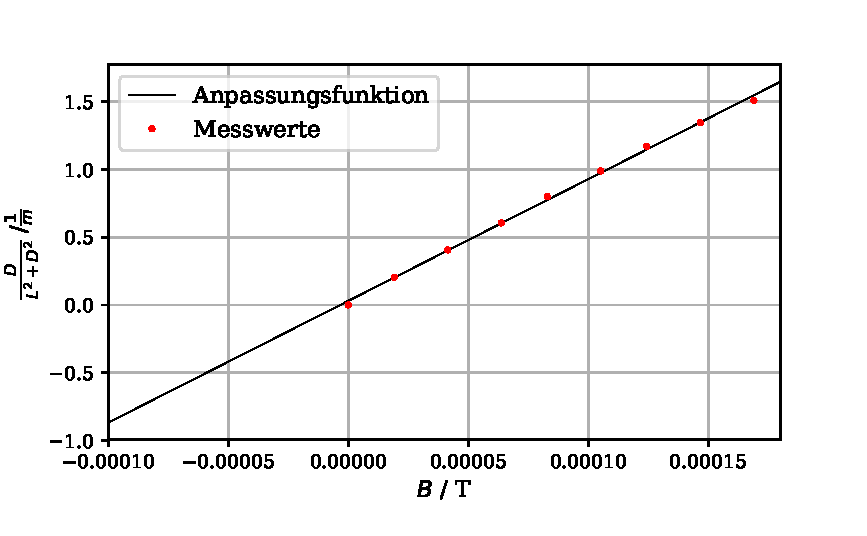
\includegraphics{plot1.pdf}
  \caption{}
  \label{fig:plot}
\end{figure}

Die lineare Ausgleichsrechnung $y = mx+C$ hat die Form
\begin{align*}
    \frac{D}{(L^2+D^2)} = \frac{1}{\sqrt{8U_B}}\sqrt{\frac{e_0}{m_0}} \cdot B + C .
\end{align*}

Es ergeben sich die Parameter
\begin{align*}
    m =
\end{align*}

Aus der Steigung berechnet man mit Hilfe von Formel () den Wert für $\frac{e_0}{m_0}$ :


\subsection{Bestimmung der Intensität des lokalen Erdmagnetfeldes}
Die Stromstärke wurde gemessen und beträgt $I = 0,15$ \si{\ampere}.
Laut Gleichung () ergibt sich daraus eine Magnetfeldstärke von
\begin{align*}
    B = 9,566 \cdot 10^{-6}
\end{align*}
Der gemessene Inklinationswinkel beträgt $\phi = 80°$.
Die Totalintensität des Erdmagnetfelds beträgt also
\begin{align*}
    B_{total} = \frac{B}{cos(\phi)} = -8,666 \cdot 10^{-5}
\end{align*}
